%----------------------------------------------------------------------------------------
%	STEP BY STEP
%----------------------------------------------------------------------------------------

\textit{Ce projet repose sur l'aide de Mathieu Hebert, en particulier de son ouvrage "Optical Models for Material Appearance", celui-ci étant disponible à la bibliothèque de l'Institut d'Optique.
}
\section{Introduction}

On se propose dans ce projet d'analyser une image contenant un ColorChecker SG, extraire les valeurs de couleur de chaque carré de la mire, et utiliser ces informations pour corriger les couleurs de l’image. Les valeurs de références fournies par le constructeur de la ColorChecker SG nous serviront de guide pour cette correction.

\medskip

Ci-dessous une représentation d'une mire ColorChecker SG. Les patches colorés sont de qualité colorimétrique, c'est-à-dire que leur couleur est très bien calibrée et connue. On note que cette mire possède un aspect \textit{glossy} (\textit{a contrario} d'une mire matte), il faut donc faire attention à ce que les sources ne reflètent de manière spéculaire lors de la prise d'image. 
Par ailleurs, ce type de mire est particulièrement onéreuse (de l'ordre de 500€), il ne faut donc en \textbf{aucun cas toucher les patches colorés. Merci de manipuler la mire avec un grande précaution}. 

\begin{center}
	\includegraphics[width=5cm]{ \dirName /images/CC_SG.jpg}
\end{center}


\section{Objectifs}
L'objectif est d'extraire les couleurs de chaque patch de la mire à partir d'une image. On va ensuite déterminer numériquement la transformation qu'il faut appliquer aux couleurs de l'image (à l'aide d'une matrice de transfert) pour que les couleurs soient fidèles à celle que l'on observe dans la réalité. 

Vous pouvez demander au LEnsE à utiliser la mire pour prendre vos propres photos, mais pour que l'effet de la correction soit perceptible, il faut que les conditions soient assez extrêmes (les smartphones font majoritairement de bonnes photos actuellement).  

%Pour cela on peut utiliser les couleurs de références de chaque patch qui nous sont fournies par le constructeur de la mire (Calibrite, anciennement X-rite), ces couelurs sont donne en CIELAB. 
Ci-dessous, une illustration du résultat qui peut être obtenu. 

\begin{center}
	\includegraphics[width=12cm]{ \dirName /images/Resultatattendu.png}
\end{center}

%%%%%%%%%%%%%%%%%%%%%%%
\section{Grandes étapes}

\begin{itemize}
	\item Définir une classe \texttt{Couleur} (qui stocke une couleur et permet d'effectuer des conversions entre les différents espaces de couleurs (sRGB, CIELAB, XYZ))
	\item Définir une classe pour représenter un patch de couleur (avec sa position, son nom et une \texttt{Couleur})
	\item Définir un système de géométries (point, quadrilatère, rectangle, grille de rectangles...). 
	\item Définir une classe de base pour représenter une ColorChecker générique :  \texttt{ColorCheckerBaseClass} (qui contiendra l'ensemble des rectangles colorés)
	\item Définir deux sous classes (qui héritent \texttt{ColorCheckerBaseClass}) : 
	\begin{itemize}
		\item Une pour représenter une ColorChecker de référence (en lisant les valeurs Lab constructeur)
		\item Une pour représenter une ColorChecker à mesurer (en analysant une image)
	\end{itemize}
	\item Définir une classe pour corriger une image à partir de deux instances de ColorChecker (une référence et une de mesure)
\end{itemize}

\medskip

\textit{Il est recommandé de monitorer visuellement l'avancée de votre projet à chaque étape. Pour cela, vous pouvez implémenter des méthodes (\texttt{.plot(self, ax = None)}) dans vos classes.}

\subsection{Focus sur l'extraction des couleurs}
L'extraction de la couleur de chaque patch peut être particulièrement  fastidieuse. On propose ici une marche à suivre générale pour simplifier le problème. 

Lors de la prise d'image, il n'y a aucune raison que la mire soit parfaitement alignée sur la grille de pixels. On peut donc penser transformer la géométrie de l'image pour que la grilles de patches colorés soit alignée sur la grille de pixels : cela simplifiera le processus de d'extraction. Les figures (a) et (b) de la figure \ref{perspective} montrent un exemple sur une image réelle. 

\begin{figure}[h]
	\centering
	\begin{subfigure}[c]{0.4\textwidth}
		\centering
		\includegraphics[width=\textwidth]{\dirName /images/corners.png}
		\caption{Représentation de la zone d'intérêt définie par les coins de la mire (sur les croix)}
		\label{distoredImage}
	\end{subfigure}
	\hfill
	\begin{subfigure}[c]{0.37\textwidth}
		\centering
		\includegraphics[width=\textwidth]{\dirName /images/unwraped.png}
		\caption{Image alignée avec la une grille de pixels. Les zones d'intérêt de chaque patch sont illustrées par des rectangles.}
		\label{undistoredImage}
	\end{subfigure}

\caption{Illustration de la transformation géométrique à appliquer sur l'image pour l'aligner}
\label{perspective}
\end{figure}

En pratique, on peut utiliser la bibliothèque \texttt{open-cv} pour réaliser cette opération, en particulier avec les fonctions \texttt{warpPerspective} et \texttt{getPerspectiveTransform}. 
Une fois l'image corrigée de sa perspective, on peut définir une grille de rectangle uniformément repartie. \textit{A fortiori}, il est intéressant d'implémenter une méthode dans les géométries afin de recadrer une image selon un rectangle. La couleur moyenne de cette sous-image peut être déterminée avec \texttt{np.mean(cropped\_img, axis = 2)}


%%%%%%%%%%%%%%%%%%%%%%%
\section{Notions utiles de colorimétrie}

\subsection{Espaces de couleur}

Les espaces colorimétriques sont des systèmes de représentation des couleurs visibles par l'œil humain. Il en existe plusieurs, selon le contexte et le but de la manipulation des couleurs. Dans ce projet, on va se focaliser principalement sur 4 notions importantes :
\begin{itemize}
\item  \textbf{sRGB} : c'est un système de couleurs (défini par la norme Rec.709) pour les écrans, les scanners et les imprimantes. Il est utilisé pour coder la grande majorité des images numérique (au format jpeg).
\item  \textbf{RGB} : c'est un espace basé sur les trois couleurs primaires : rouge, vert et bleu. Il existe une infinité de variantes de RGB, selon le blanc de référence et les coordonnées chromatiques des trois couleurs utilisées comme primaires pour le système. Il existe l'espace CIERGB qui est un espace RGB défini par un point blanc et trois valeurs particulière de couleurs primaires. 

\begin{itemize}
	\item Il est important de ne pas faire de confusion entre le sRGB et RGB. En particulier, le lien entre les deux n'est pas linéaire. Le sRGB est encodé avec une non-linéarité par rapport aux valeurs de luminances affichées (pour reproduire le comportement de l'œil et optimisé le stockage) que l'on appelle courbe $\gamma$. 
\end{itemize}

\item  \textbf{CIELAB} : c'est un espace perceptuel, qui tient compte de la façon dont l'œil humain perçoit les couleurs. Il se compose de trois axes : $L$ pour la luminosité, $a$ pour la teinte entre rouge et vert, et $b$ pour la teinte entre jaune et bleu. Aussi appelé $L$*$a$*$b$* CIE 1976. Voir figure \ref{Lab}.
\item \textbf{XYZ} : c'est un espace normalisé par la Commission Internationale de l'Eclairage (CIE), qui englobe toutes les couleurs visibles par l'œil humain. Il se base sur les fonctions colorimétriques $\bar{x}(\lambda)$, $\bar{y}(\lambda)$ et $\bar{z}(\lambda)$, qui mesurent la réponse des cônes de la rétine à différentes longueurs d'onde. Voir figure \ref{XYZ}.

\begin{figure}[h]
	\centering
	\begin{subfigure}[b]{0.4\textwidth}
		\centering
		\includegraphics[width=\textwidth]{\dirName /images/Chromaticity_Diagram.png}
		\caption{CIE 1931 XYZ}
		\label{XYZ}
	\end{subfigure}
	\hfill
	\begin{subfigure}[b]{0.59\textwidth}
		\centering
		\includegraphics[width=\textwidth]{\dirName /images/Lab-color-space.jpg}
		\caption{$L$*$a$*$b$* CIE 1976}
		\label{Lab}
	\end{subfigure}

\caption{Représentations graphiques d'espaces colorimétriques}
\label{fig:three graphs}
\end{figure}


\end{itemize}


\subsubsection{Conversion d'espaces de couleur}
La conversion d'un espace de couleur à un autre repose sur des transformations mathématiques standardisées, ces opérations sont assez pénibles à implémenter (et ce n'est pas l'idée du travail à effectuer). 
Il existe des bibliothèques Python qui permettent de convertir les espaces de couleurs, on peut recommander :
\begin{itemize}
	\item \texttt{skimage.color} : bien documenté et très simple d'utilisation. La figure \ref{conversion}, illustre les fonctions utiles dans notre cas. 
	\item \texttt{colour-science} : Très bien documenté et très complet. Mais il y a énormément de fonctionnalités très avancées qui ne sont pas utiles, on peut vite s'y perdre.
	\item \texttt{open-cv} : Bibliothèque très riche avec une grande communauté d'utilisateurs, mais les documentations est parfois assez abrupte (car adaptée du C++).  
\end{itemize}

\begin{figure}[h]
	\centering
		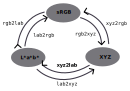
\includegraphics[width=.4\textwidth]{\dirName /images/conversion.png}
		\caption{Diagramme des fonctions de conversion disponibles dans \texttt{skimage.color}. Notez que pour cette bibliothèque \texttt{rgb} représente le sRGB.}
	\label{conversion}
\end{figure}

%%%%%%%%%%%%%%%%%%%%%%%
\subsection{Correction colorimétrique}

\subsubsection{Calcule de la matrice de correction}
Pour chaque patch coloré (ici indexé par $j \in [\![ 1, N  ]\!]$) de la mire, on cherche à résoudre l'équation matricielle : 

\begin{equation}
    \begin{bmatrix}
        X_j^\text{ref} & Y_j^\text{ref}  & Z_j^\text{ref} \\
    \end{bmatrix}
    =  w_j^T \cdot U
	\label{equation matriciel simple}
\end{equation}

Le vecteur $[X_j^\text{ref} \, Y_j^\text{ref} \, Z_j^\text{ref}]$ représente les coordonnées colorimétriques fournies par le constructeur de la mire dans l'espace CIE 1931 XYZ pour le patch $j$. 

Le vecteur $w_j$ est une combinaison polynômes des valeurs $\left( X_j, Y_j, Z_j \right)$ mesurées sur chaque patch de l'image. Selon l'ordre de correction choisi, les valeurs de $w_j$ sont les suivantes : 

\begin{table}[h]
	\centering
	\begin{tabular}{|l|l|}
	\hline
	\textbf{Ordre 1} &
	$w_j = \left(1, X_j, Y_j, Z_j \right) $ \\ \hline
	\textbf{Ordre 2} &
	$w_j = \left(1, X_j, Y_j, Z_j, X_j^2 , X_j  Y_j, X_j  Z_j, Y_j^2, Y_j Z_j, Z_j^2   \right)$ \\ \hline
	\textbf{Ordre 3} & $w_j =$ 
	\begin{tabular}[c]{@{}l@{}}$(1, X_j, Y_j, Z_j, X_j^2 , X_j  Y_j, X_j  Z_j, Y_j^2, Y_jZ_j, Z_j^2, $\\ $X_j^3, X_j^2Y_j, X_j^2Z_j, X_jY_j^2, X_jY_jZ_j, X_j^2Z_j, Y_j^3, Y_j^2Z_j, Y_jZ_j^2, Z_j^3)$\end{tabular} \\ \hline
	\end{tabular}
\end{table}

On nomme $k$ la taille du vecteur $w_j$ (cette valeur dépend dont de l'ordre de correction choisi). La taille de la matrice $U$ sera alors $[k, 3]$. 

L'idée est donc de chercher une matrice $U$ qui transforme les valeurs $\left( X_j, Y_j, Z_j \right)$ erronées en $(X_j^\text{ref} \, Y_j^\text{ref} \, Z_j^\text{ref})$. L'usage de $w_j$ permet de d'ajouter de la surdétermination dans le système linéaire avec des termes croisés et ainsi de facilité la résolution numérique. 

Dans notre cas, il y a $N=140$ patchs sur la mire. On peut écrire de manière plus condensée le système des 140 équations matricielles \ref{equation matriciel simple} de la manière suivante : 

\begin{equation}
    \begin{bmatrix}
        X_1^\text{ref} & Y_1^\text{ref}  & Z_1^\text{ref} \\
		\vdots & \vdots & \vdots \\
		X_N^\text{ref} & Y_N^\text{ref}  & Z_N^\text{ref}
    \end{bmatrix}
    =  \begin{bmatrix}
        w_1^T \\
		\vdots  \\
		w_N^T
    \end{bmatrix} \cdot U
	\label{equation matriciel complexe}
\end{equation}

On peut alors trouver la matrice $U$ avec une résolution numérique basée sur la méthode des moindres carrés. La bibliothèque \texttt{scipy.linalg} dispose d'une fonction \texttt{lstsq} qui peut résoudre l'équation sous la forme de l'équation \ref{equation matriciel complexe}. C'est-à-dire avec une matrice de gauche de dimension $[140, 3]$, une matrice contenant les $w_k$ de taille $[140, k]$ et toujours une matrice $U$ de dimension $[k, 3]$. 

\subsubsection{Correction de l'image}

Après avoir calculé la matrice de correction $U$, il est possible de corriger le rendu colorimétrique de l'image. On doit disposer de l'image convertie en coordonnées XYZ, cette image est représentée par une matrice de taille $[H, W, 3]$, ou $H$ et $W$ sont respectivement la hauteur et largeur de l'image.
\medskip
L'idée est d'utiliser cette image pour créer une matrice $\tilde{M}_\text{img}$ de taille $[H, W, k]$ (où $k$ est la taille du vecteur $w+j$). Sur sa troisième dimension, cette matrice aura la même valeur que le polynôme qui représente $w_j$. Ci-dessous une image pour illustrer la matrice que l'on veut obtenir. En pratique, pour construire cette matrice avec Python, il peut être intéressant d'utiliser les fonctions \texttt{stack}, \texttt{concatenate} et \texttt{squeeze} de la bibliothèque \texttt{numpy}.

\begin{center}
	
\includegraphics[width=7cm]{ \dirName /images/schema matrice.png}
\end{center}

Pour appliquer la correction, il est possible de faire le produit matriciel entre $\tilde{M}_\text{img}$ et $U$ sans passer par une boucle. En effet, la fonction \texttt{dot} de \texttt{numpy} gère la matrice à trois dimensions, le résultat de cette opération sera une image corrigée en XYZ de taille $[H, W, 3]$. Pour afficher l'image, il faut finalement convertir l'image en sRGB. 


%%%%%%%%%%%%%%%%%%%%%%%
\section{Quelques pistes d'ouvertures possibles}

\textbf{Vous devrez choisir et réaliser au moins l'une des ouvertures suivantes dans le cadre de ce projet}.

\begin{description}

	\item[Ouverture A] \textbf{Impact de l'ordre de correction}
	
	\begin{itemize}
		\item Il est possible d'étudier visuellement l'impact de l'ordre choisi sur $w_j$ sur la qualité de correction. 
	\end{itemize}	

\qquad

	\item[Ouverture B] \textbf{Graphes de modification de la chromaticité $xy$}

	
	\begin{itemize}
		\item Il est possible de réaliser un graphe dans le diagramme de chromaticité CIE 1931 xy; pour chaque patch on peut tracer une flèche qui illustre la modification de chromaticité entre la référence et l'image, avant et après correction. 
	\end{itemize}	

\qquad
	
	\item[Ouverture C] \textbf{Detection automatique de la mire}
	\begin{itemize}
		\item Il existe des librairies Python qui permettent de détecter automatiquement les mires type ColorChecker dans une image. Cela évite de devoir renseigner manuellement les coordonnées des 4 coins de la mire. Voir : \href{https://www.colour-science.org/colour-checker-detection/}{Site de colour-science pour la détection de ColorCheckers}
	\end{itemize}
	
\end{description}


%%%%%%%%%%%%%%%%%%%%%%%%%
\section{Critères d'évaluation}

\textbf{Grille à simplifier (bilan Semestre 5)}

\begin{itemize}
	\item \textbf{METHODES NUMERIQUE}
	\begin{itemize}
		\item \textbf{Ecriture Matricielle / Vectorielle}
		\begin{itemize}
			\item utilisation des méthodes liées aux vecteurs/matrices (Numpy)
			\item aucune boucle \textbf{for} inutile
		\end{itemize}		 
		\item \textbf{Organisation en actions élémentaires}
		\begin{itemize}
			\item les étapes sont découpées en fonctionnalité plus simple à tester
		\end{itemize}
		\item \textbf{Description des tests de validation}
		\begin{itemize}
			\item chaque fonction a été testée
			\item chaque étape a été validée
		\end{itemize}
		\item \textbf{Organisation des informations à traiter}
		\begin{itemize}
			\item les données sont rangées dans des objets bien identifiés
		\end{itemize}
	\end{itemize}


	\item \textbf{PROGRAMMATION}
	\begin{itemize}
		\item \textbf{Ecriture globale du code et commentaires (PEP 8)}
		\begin{itemize}
			\item variables et fonctions respectant les conventions d'écriture standard
			\item commentaires utiles
		\end{itemize}		 
		\item \textbf{Utilisation, écriture de fonctions}
		\begin{itemize}
			\item paramètres et retours pertinents des fonctions
		\end{itemize}
		\item \textbf{Documentation des fonctions (PEP257)}
		\begin{itemize}
			\item paramètres et retours des fonctions sont documentés
		\end{itemize}
		\item Création de classes et d'objets
		\begin{itemize}
			\item classe contenant des attributs et méthodes pertinents
			\item aucune fonction n'est appelée en dehors d'un objet
		\end{itemize}
	\end{itemize}
	

	\item \textbf{INGENIEUR.E PHYSIQUE}
	\begin{itemize}
		\item \textbf{Graphiques pertinents et légendés}
		\begin{itemize}
			\item graphiques scientifiques (axes, titre...)
			\item axes des graphiques légendés (passage temps/fréquence)
		\end{itemize}		 
		\item \textbf{Organisation en actions élémentaires}
		\begin{itemize}
			\item les étapes sont découpées en fonctionnalité plus simple à tester
		\end{itemize}
		\item \textbf{Génération de données pertinentes de tests}
		\begin{itemize}
			\item choix de la position des sources pertinent
		\end{itemize}
		\item \textbf{Analyse des données et validation modèle}
		\begin{itemize}
			\item comparaison avec la théorie
			\item analyse pertinente des cartes obtenues
		\end{itemize}
	\end{itemize}
	
\medskip	
	
	\item \textbf{AVANCEMENT}
	\begin{itemize}
		\item Étapes 1 et 2 : x 0.5
		\item Étapes 1, 2 et 3 : x 0.7
		\item Une des ouvertures : x 1.0
	\end{itemize}
\end{itemize}



